% Please remember only one sentence per line!
\section{Results}
% TODO: Present the results.

\subsection{Decision rule accuracies}
Figure \ref{fig2} shows the accuracy of each decision rule against the choices made by participants in the experiment (on the x-axis) and the accuracy against the growth rate optimal choices.
% What does the figure show?
Each decision rule is represented by a colour.
There are 58 dots per decision rule, each dot representing a participant in the experiment.
There is a large spread in how well the decision rules approximates the choices across participants.
Variation across the participants within each colour along the y-axis stems from differences in the gamble pairs to which the participants were exposed.
Variation along the x-axis stems from differences in the actual choices made by each participant.

The figure shows that the simplest decision rules, like avoiding the worst fractal or giving preference to the best, do not predict choices better than random (the dots cluster around a choice accuracy of 0.5).
Furthermore, they are also no better than random choice in terms of growth rate maximization.
This is true for both the additive and multiplicative dynamic.

The decision rule based on the sign cue is somewhat better in terms of accurately predicting experimental choices. However, it does not predict choices as well as the priority heuristic (and variations). Neither does it deliver growth rate optimality.

\begin{figure}
    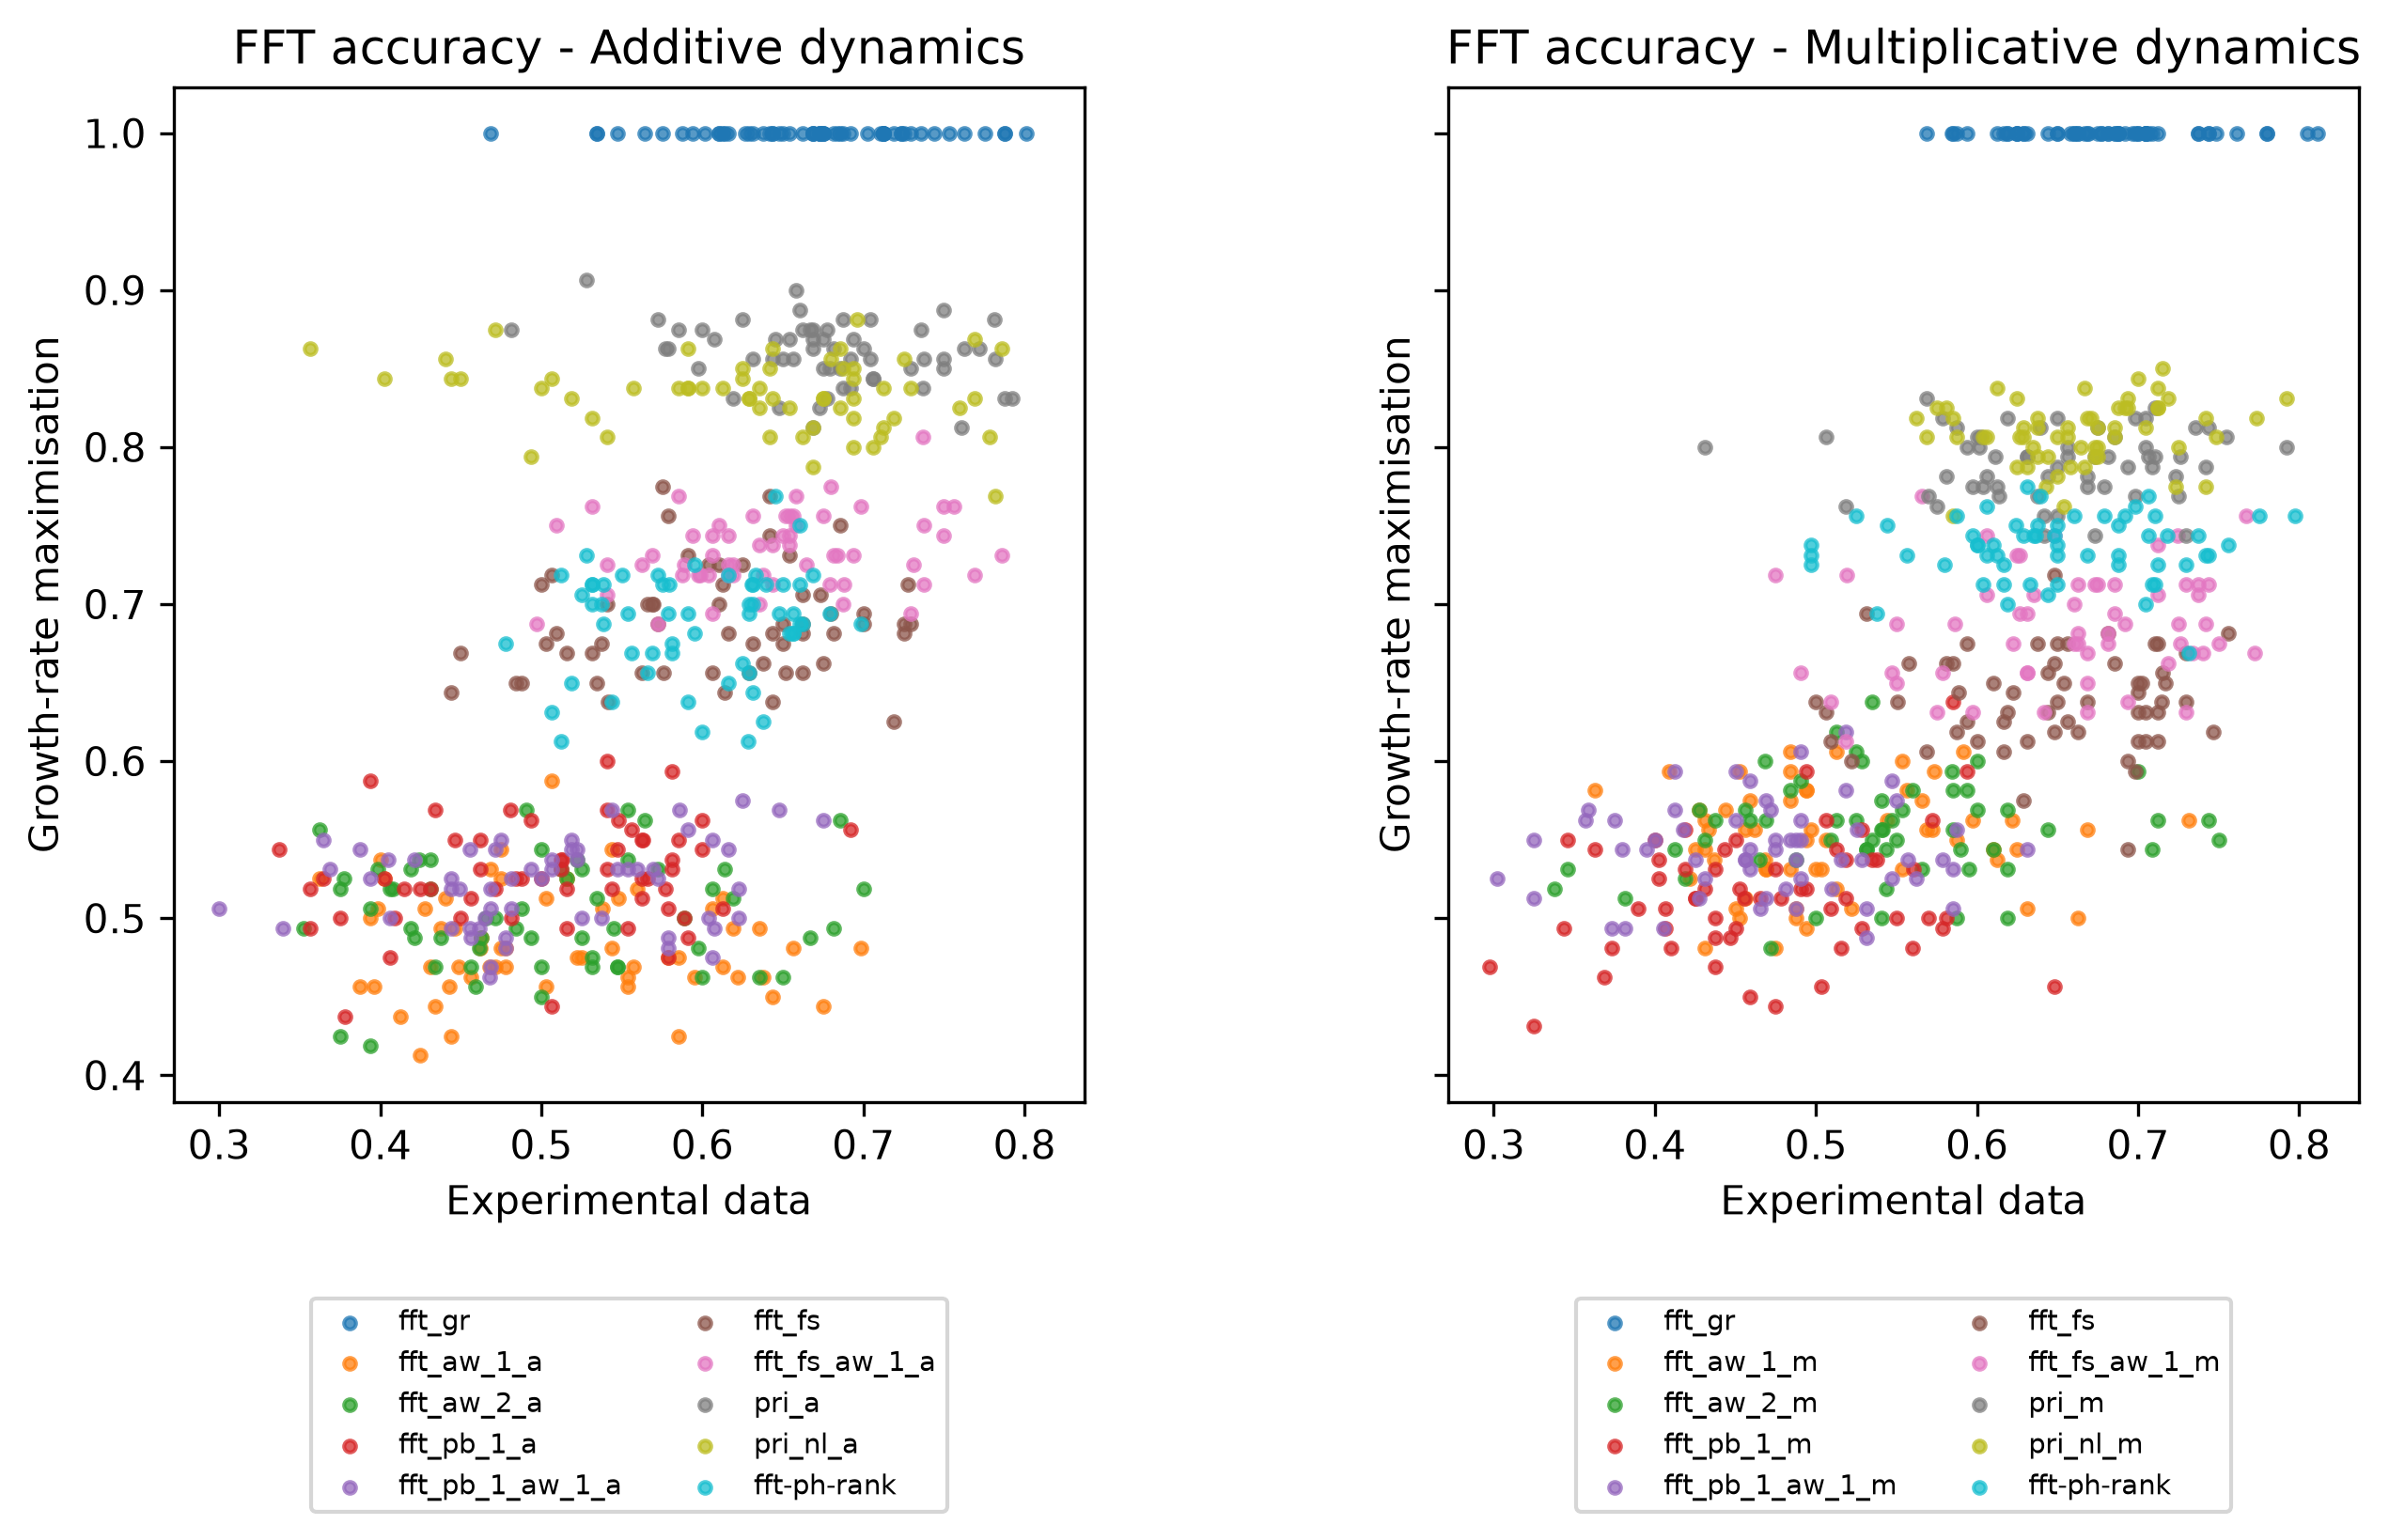
\includegraphics[width=1.0\textwidth]{figures/fig2.png}
    \label{fig2}
    \caption{Decision rule accuracy against experimental results (x-axis) and growth rate optimal choices (y-axis) for each participant in the experiment.}
\end{figure}

The accuracies are summarized in Table \ref{tab:accuracy}.
There seem to be no better predictor of actual choices than growth rate optimality.
The priority heuristic predicts choices as well, but not better.
Perhaps its success is because it approximates the growth-rate optimality well?

The table also shows the importance-weighted accuracy score.
The importance-weighted accuracy indicates how close to the optimal growth rate an agent can achieve by applying the decision rule.

The sign rule and the priority heuristics have very high importance-weighted accuracy, implying that even if there are some choices where they fail to make the growth optimal decision, they still manage to achieve near optimal growth rate.
That is, they get the important choices right.

\begin{table}[htbp]
    \centering
    \caption{Mean accuracy and range for each FFT.
    ACC: Accuracy (average match rate) between GR and choices.
    WACC: Importance-weighted accuracy between GR and choices.
    CACC: Accuracy between experimental choices and decision rules. }
    \label{tab:accuracy}
    \begin{tabular}{lccc}
FFT & acc & wacc & cacc \\
additive \\
fft\_gr &  &  & 0.66 [0.47 - 0.79] \\
fft\_aw\_1\_a & 0.48 [0.41 - 0.59] & 0.43 [0.32 - 0.56] & 0.51 [0.36 - 0.69] \\
fft\_aw\_2\_a & 0.5 [0.42 - 0.57] & 0.48 [0.38 - 0.58] & 0.5 [0.35 - 0.7] \\
fft\_pb\_1\_a & 0.53 [0.44 - 0.6] & 0.56 [0.48 - 0.63] & 0.5 [0.34 - 0.69] \\
fft\_pb\_1\_aw\_1\_a & 0.52 [0.46 - 0.57] & 0.51 [0.41 - 0.59] & 0.5 [0.3 - 0.68] \\
fft\_fs & 0.69 [0.62 - 0.78] & 0.83 [0.78 - 0.89] & 0.61 [0.44 - 0.72] \\
fft\_fs\_aw\_1\_a & 0.73 [0.69 - 0.81] & 0.86 [0.82 - 0.92] & 0.64 [0.49 - 0.78] \\
pri\_a & 0.86 [0.81 - 0.91] & 0.97 [0.95 - 0.98] & 0.67 [0.48 - 0.79] \\
pri\_nl\_a & 0.83 [0.77 - 0.88] & 0.95 [0.93 - 0.97] & 0.63 [0.36 - 0.78] \\
fft-ph-rank & 0.69 [0.61 - 0.77] & 0.82 [0.72 - 0.86] & 0.59 [0.48 - 0.69] \\
experiment\_a & 0.66 [0.47 - 0.79] & 0.76 [0.45 - 0.88] &  \\
multiplicative \\
fft\_gr &  &  & 0.67 [0.56 - 0.81] \\
fft\_aw\_1\_m & 0.55 [0.48 - 0.61] & 0.57 [0.5 - 0.65] & 0.51 [0.36 - 0.73] \\
fft\_aw\_2\_m & 0.56 [0.48 - 0.64] & 0.6 [0.52 - 0.69] & 0.54 [0.34 - 0.75] \\
fft\_pb\_1\_m & 0.51 [0.43 - 0.64] & 0.51 [0.42 - 0.6] & 0.47 [0.29 - 0.64] \\
fft\_pb\_1\_aw\_1\_m & 0.54 [0.49 - 0.62] & 0.55 [0.47 - 0.64] & 0.47 [0.3 - 0.63] \\
fft\_fs & 0.64 [0.54 - 0.72] & 0.76 [0.67 - 0.82] & 0.64 [0.5 - 0.76] \\
fft\_fs\_aw\_1\_m & 0.69 [0.61 - 0.77] & 0.8 [0.71 - 0.86] & 0.65 [0.48 - 0.76] \\
pri\_m & 0.79 [0.74 - 0.83] & 0.89 [0.86 - 0.93] & 0.65 [0.43 - 0.79] \\
pri\_nl\_m & 0.81 [0.76 - 0.85] & 0.93 [0.89 - 0.95] & 0.66 [0.56 - 0.79] \\
fft-ph-rank & 0.74 [0.67 - 0.78] & 0.89 [0.84 - 0.91] & 0.65 [0.49 - 0.79] \\
experiment\_m & 0.67 [0.56 - 0.81] & 0.77 [0.62 - 0.93] &  \\
\end{tabular}

\end{table}

\subsection{$\eta$-profiles}
The $\eta$-profiles, plotted in Figure \ref{fig4} measure the accuracy of a decision rule against expected utility maximisation for different values of $\eta$. 
The $\eta$ value that gives the maximum accuracy (the peak of the profile) indicates good estimates of the apparent risk-preference parameter.
The profiles of the actual choices peak around 0 in the additive dynamics, and around 1 in the multiplicative.

The figure shows that the simple heuristics such as avoid the worst and prefer the best result in profiles that are completely different from the experimental data.
Avoid the worst implies an apparent $\eta >5$, which is much higher than that of the experimental data. 
The decision rule therefore implies a high degree of risk aversion that is not present in the data.
The opposite is true for prefer the best heurstic.
It implies an apparent $\eta<-1$, while such risk-seeking was not present in the experimental data.

Even though the sign-based heuristic was fairly good at predicting choices, it does not result in an $\eta$-profile that resembles the observational data.
For the additive case, the apparent $\eta$ is too low  (<0) and for the multiplicative case it is too high (around 1.7). 
Hence, the sign-based heuristic cannot explain the observed data.

In the additive case, the priority heuristic results in a profile that is similar to the data (and to growth rate optimality), peaking around 0.
However, in the multiplicative case the profile of the no loss version is closer.

\begin{figure}
    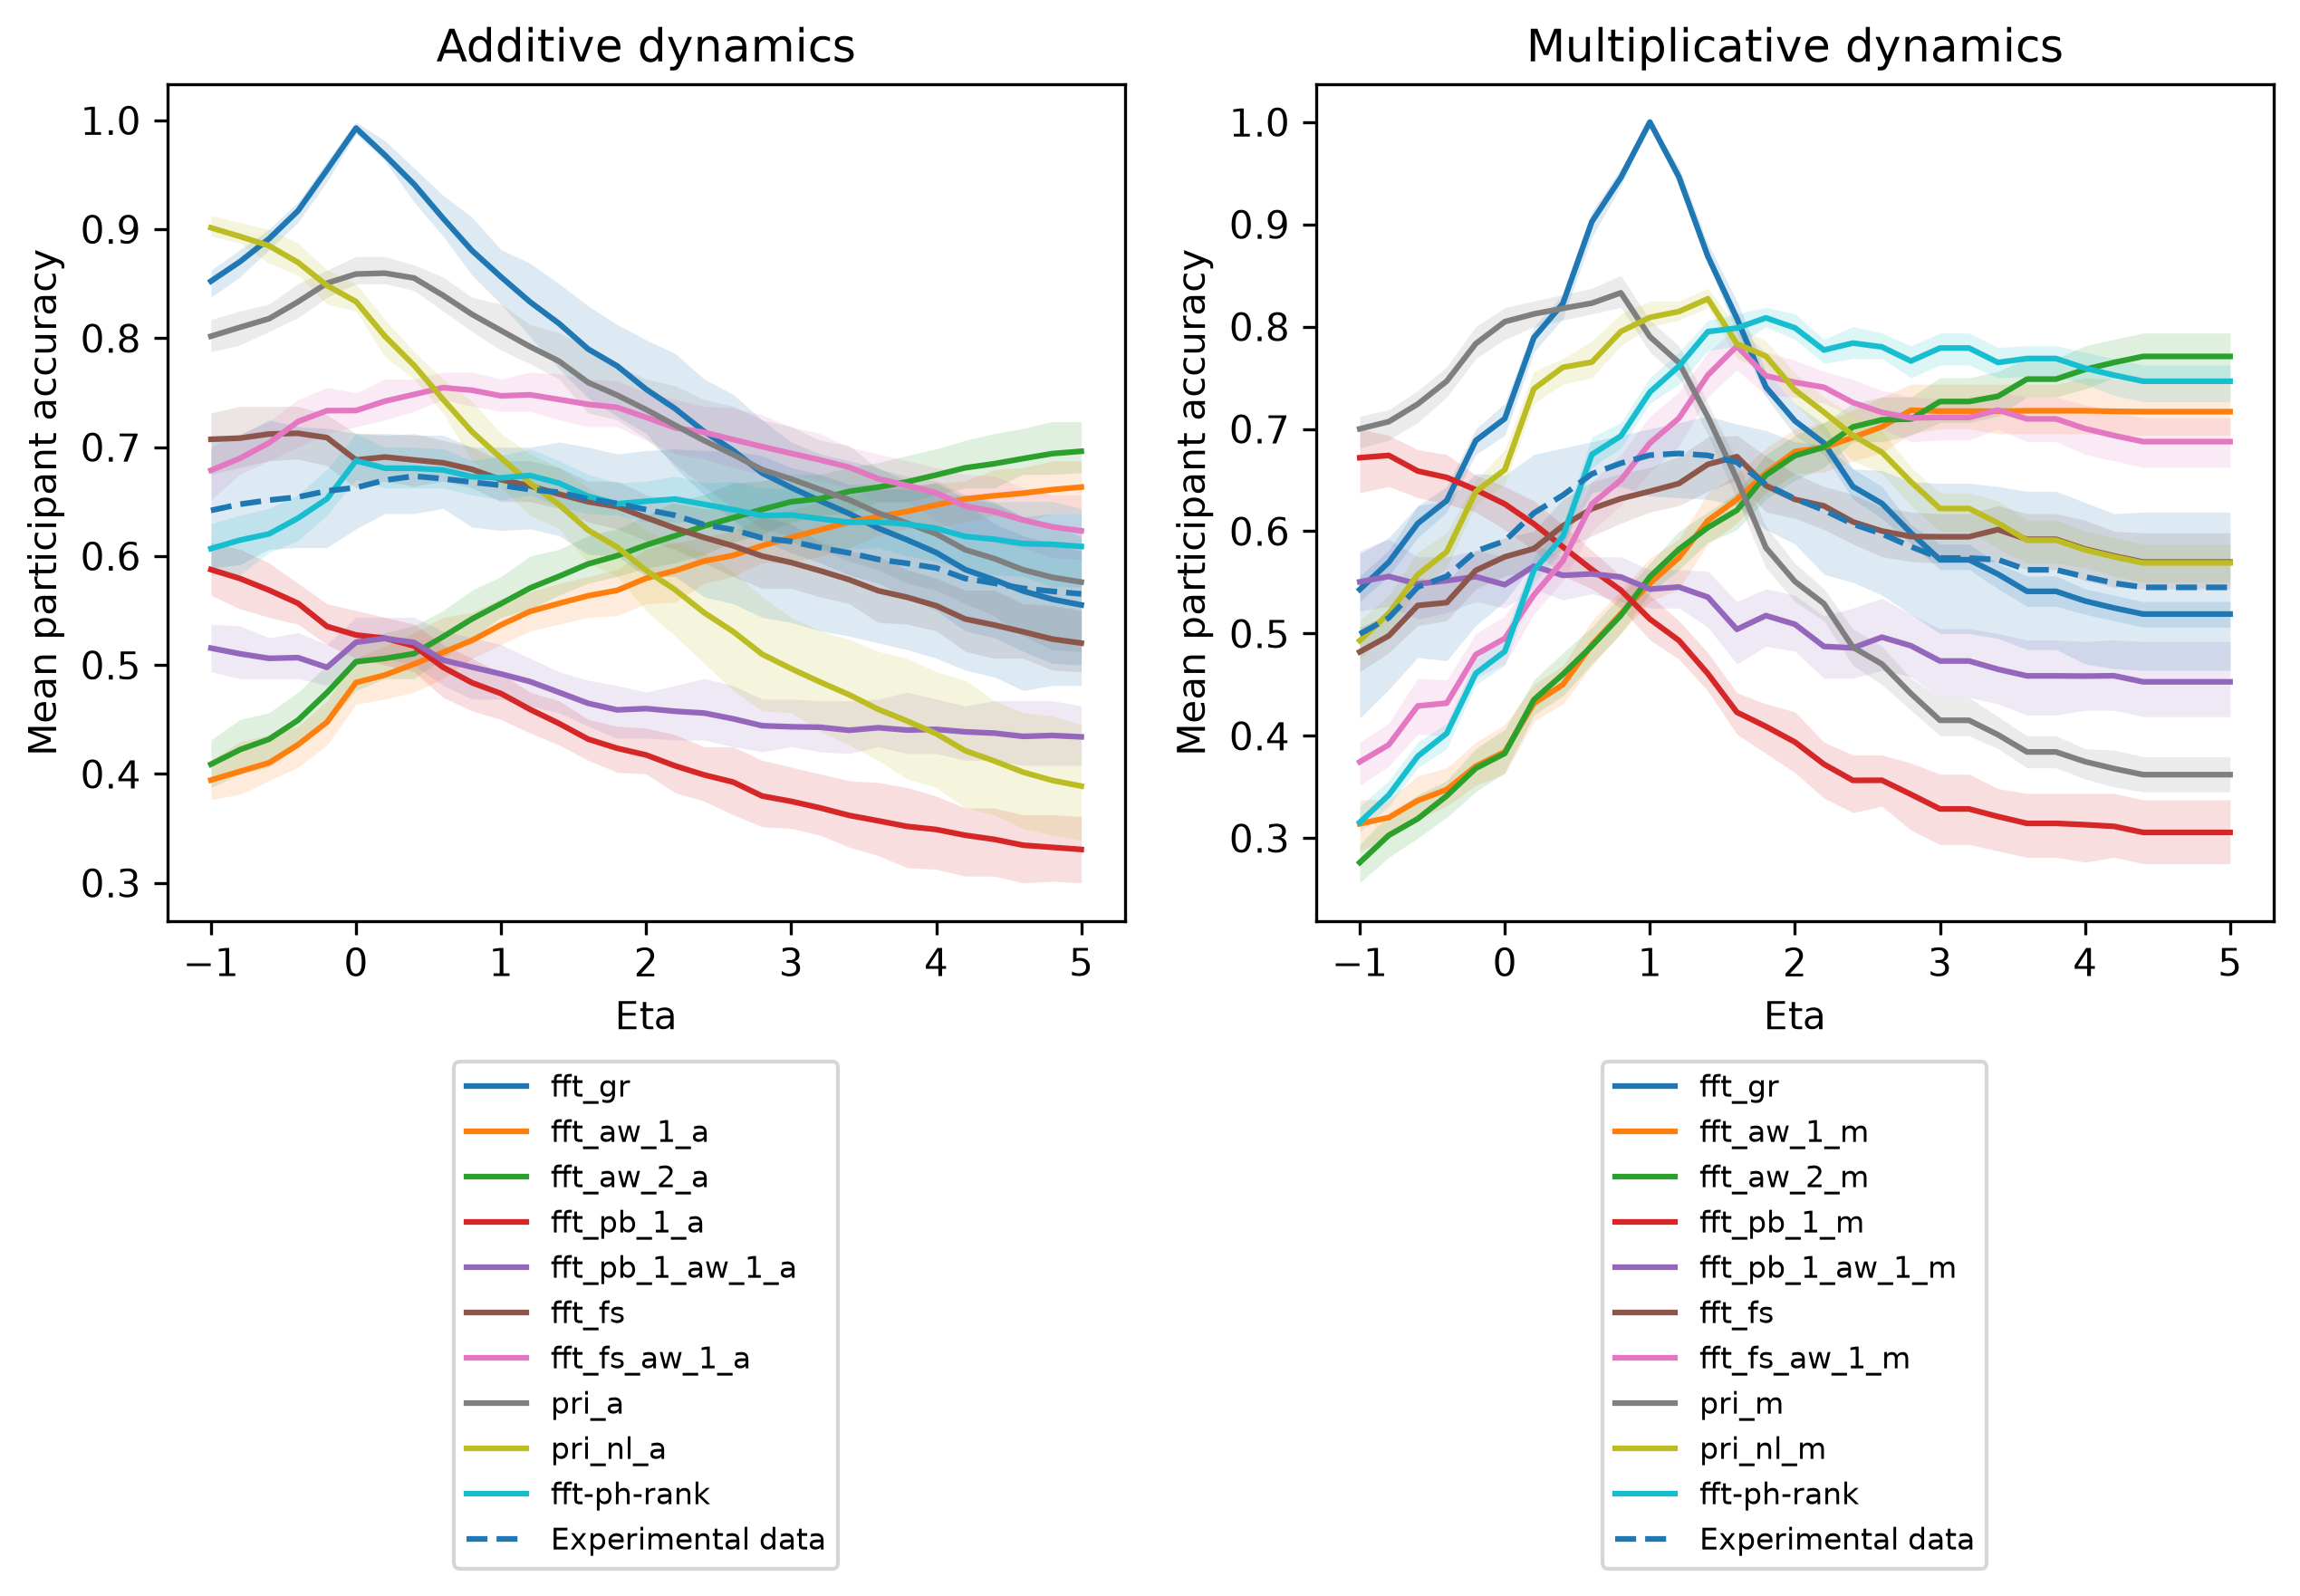
\includegraphics[width=1.0\textwidth]{figures/fig4.png}
    \label{fig4}
    \caption{$\eta$-profiles: The profile shows the decision rule accuracy against an expected utility maximizer with a given risk preference (expressed as $\eta$ along the x-axis).
    The lines mark the mean across all experiment participants and the shared areas represent the central interquartile band (25th–75th percentile).}
\end{figure}